\documentclass{article}
\usepackage[table]{xcolor}
\usepackage{tikz}
\usetikzlibrary{arrows.meta,positioning,calc,decorations.pathreplacing}
\usepackage{listings}
\usepackage[most]{tcolorbox}
\usepackage{booktabs}
\usepackage{array}
\usepackage[default]{sourcesanspro}
\usepackage[scale=0.88]{sourcecodepro}
\definecolor{gblue}{HTML}{4285F4}
\definecolor{gred}{HTML}{EA4335}
\definecolor{gyellow}{HTML}{F9AB00}
\definecolor{ggreen}{HTML}{34A853}
\definecolor{blue700}{HTML}{1967D2}
\definecolor{green700}{HTML}{188038}
\definecolor{red700}{HTML}{C5221F}
\definecolor{yellow800}{HTML}{B0740A}
\definecolor{ink}{HTML}{202124}
\definecolor{gray7}{HTML}{5F6368}
\definecolor{gray5}{HTML}{9AA0A6}
\definecolor{gray3}{HTML}{DADCE0}
\definecolor{codebg}{HTML}{F8F9FA}
\definecolor{purple}{HTML}{9334E6}
\definecolor{regteal}{HTML}{0F766E}
\definecolor{dirpurple}{HTML}{7C5CB0}
\tikzset{
  slot/.style={draw=gray5, line width=0.6pt, minimum width=4.9cm,
               minimum height=0.72cm, font=\small, inner sep=2pt},
  addrlbl/.style={font=\footnotesize\ttfamily\color{gray7}},
  sidelbl/.style={font=\footnotesize\color{gray7}},
  flowarrow/.style={-{Stealth[length=2.6mm]}, line width=1pt},
  cyclenode/.style={rounded corners=3pt, line width=0.8pt, minimum width=3.1cm,
                    minimum height=0.95cm, font=\small\bfseries, text=ink},
}
\begin{document}
\section*{Guide figures}

\subsection*{memory}
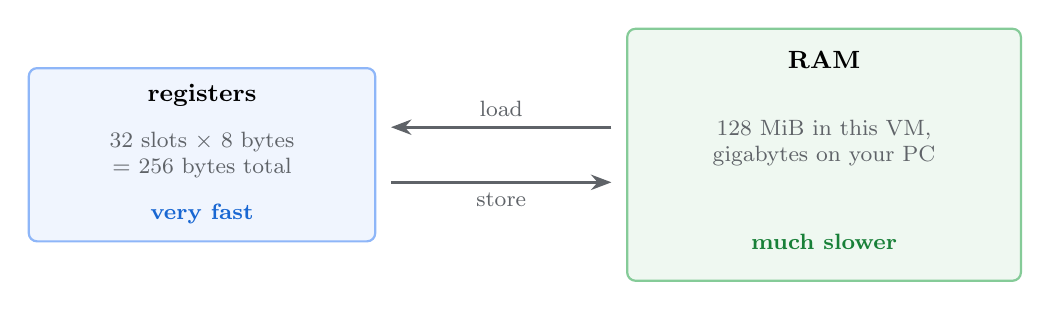
\begin{tikzpicture}[x=1cm,y=1cm]
  % registers card
  \draw[rounded corners=3pt, fill=gblue!8, draw=gblue!60, line width=0.8pt]
    (0,0) rectangle (4.4,2.2);
  \node[font=\small\bfseries] at (2.2,1.85) {registers};
  \node[font=\footnotesize\color{gray7}, align=center] at (2.2,1.1)
    {32 slots $\times$ 8 bytes\\ = 256 bytes total};
  \node[font=\footnotesize\bfseries\color{blue700}] at (2.2,0.35) {very fast};
  % ram card
  \draw[rounded corners=3pt, fill=ggreen!8, draw=ggreen!60, line width=0.8pt]
    (7.6,-0.5) rectangle (12.6,2.7);
  \node[font=\small\bfseries] at (10.1,2.3) {RAM};
  \node[font=\footnotesize\color{gray7}, align=center] at (10.1,1.25)
    {128 MiB in this VM,\\ gigabytes on your PC};
  \node[font=\footnotesize\bfseries\color{green700}] at (10.1,0.0) {much slower};
  % arrows: load reads memory into a register, store writes a register out to memory
  \draw[flowarrow, gray7] (7.4,1.45) -- node[above,font=\footnotesize]{load} (4.6,1.45);
  \draw[flowarrow, gray7] (4.6,0.75) -- node[below,font=\footnotesize]{store} (7.4,0.75);
\end{tikzpicture}

\subsection*{the_stack_and_the_heap}
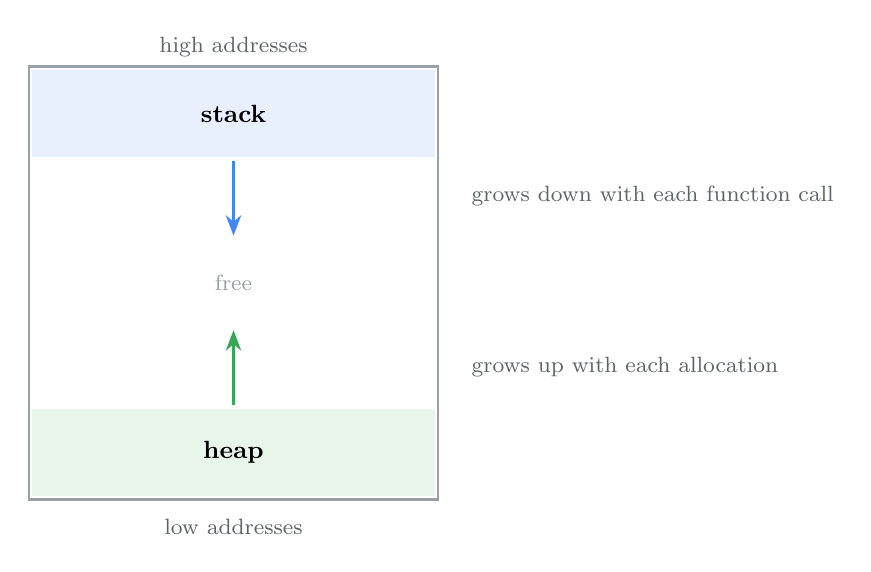
\begin{tikzpicture}[x=1cm,y=1cm]
  \node[sidelbl] at (2.6,5.75) {high addresses};
  \draw[gray5, line width=0.8pt] (0,0) rectangle (5.2,5.5);
  % stack band
  \fill[gblue!12] (0.04,4.35) rectangle (5.16,5.46);
  \node[font=\small\bfseries] at (2.6,4.9) {stack};
  \draw[flowarrow, gblue] (2.6,4.3) -- (2.6,3.35);
  \node[sidelbl, anchor=west] at (5.5,3.85) {grows down with each function call};
  % heap band
  \fill[ggreen!12] (0.04,0.04) rectangle (5.16,1.15);
  \node[font=\small\bfseries] at (2.6,0.6) {heap};
  \draw[flowarrow, ggreen] (2.6,1.2) -- (2.6,2.15);
  \node[sidelbl, anchor=west] at (5.5,1.68) {grows up with each allocation};
  % free space
  \node[font=\footnotesize\color{gray5}] at (2.6,2.75) {free};
  \node[sidelbl] at (2.6,-0.35) {low addresses};
\end{tikzpicture}

\subsection*{how_the_cpu_reads_instructions}
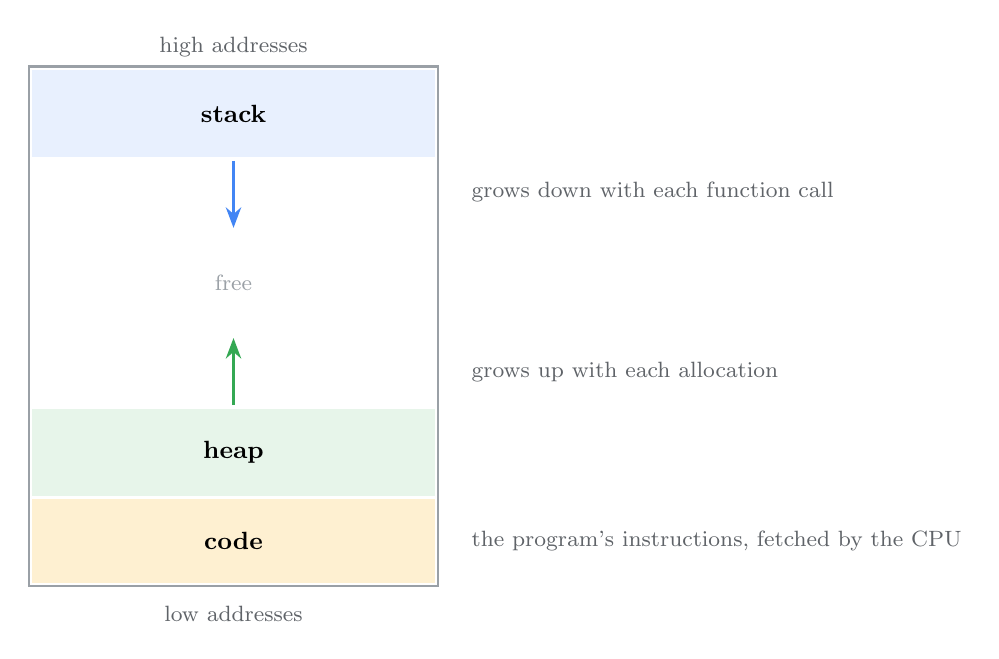
\begin{tikzpicture}[x=1cm,y=1cm]
  \node[sidelbl] at (2.6,6.85) {high addresses};
  \draw[gray5, line width=0.8pt] (0,0) rectangle (5.2,6.6);
  % stack
  \fill[gblue!12] (0.04,5.45) rectangle (5.16,6.56);
  \node[font=\small\bfseries] at (2.6,6.0) {stack};
  \draw[flowarrow, gblue] (2.6,5.4) -- (2.6,4.55);
  \node[sidelbl, anchor=west] at (5.5,5.0) {grows down with each function call};
  % heap
  \fill[ggreen!12] (0.04,1.14) rectangle (5.16,2.25);
  \node[font=\small\bfseries] at (2.6,1.7) {heap};
  \draw[flowarrow, ggreen] (2.6,2.3) -- (2.6,3.15);
  \node[sidelbl, anchor=west] at (5.5,2.72) {grows up with each allocation};
  \node[font=\footnotesize\color{gray5}] at (2.6,3.85) {free};
  % code
  \fill[gyellow!18] (0.04,0.04) rectangle (5.16,1.1);
  \node[font=\small\bfseries] at (2.6,0.57) {code};
  \node[sidelbl, anchor=west] at (5.5,0.57) {the program's instructions, fetched by the CPU};
  \node[sidelbl] at (2.6,-0.35) {low addresses};
\end{tikzpicture}

\subsection*{how_the_cpu_reads_instructions_2}
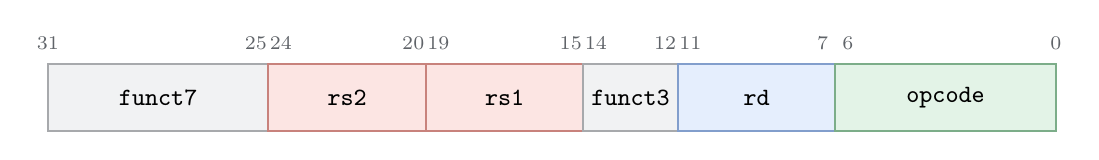
\begin{tikzpicture}[x=1cm,y=1cm]
  \newcommand{\bit}{0.40}
  % fields: name/start bit index (from left, 0..32)/width in bits/color
  % funct7: 0-7, rs2: 7-12, rs1: 12-17, funct3: 17-20, rd: 20-25, opcode: 25-32
  \foreach \name/\s/\w/\col in {funct7/0/7/gray5, rs2/7/5/gred, rs1/12/5/gred,
                                funct3/17/3/gray5, rd/20/5/gblue, opcode/25/7/ggreen} {
    \draw[fill=\col!14, draw=\col!70!black!60, line width=0.7pt]
      ({\s*\bit},0) rectangle ({(\s+\w)*\bit},0.85);
    \node[font=\small\ttfamily] at ({(\s+\w/2)*\bit},0.425) {\name};
  }
  % bit indices
  \foreach \b/\i in {0/31, 6.6/25, 7.4/24, 11.6/20, 12.4/19, 16.6/15, 17.4/14,
                     19.6/12, 20.4/11, 24.6/7, 25.4/6, 32/0}
    \node[font=\scriptsize\color{gray7}] at ({\b*\bit},1.12) {\i};
\end{tikzpicture}

\subsection*{how_the_cpu_reads_instructions_3}
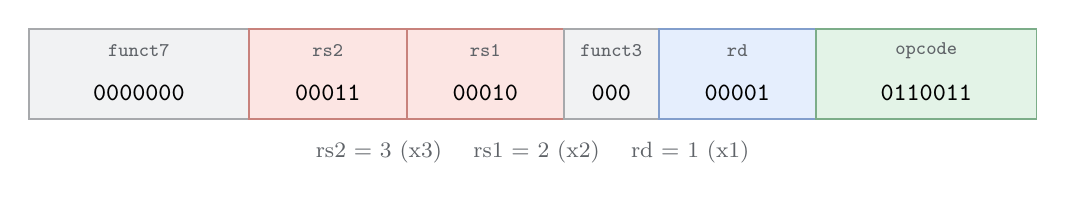
\begin{tikzpicture}[x=1cm,y=1cm]
  \newcommand{\bit}{0.40}
  % filled-in encoding
  \foreach \name/\val/\s/\w/\col in {funct7/0000000/0/7/gray5, rs2/00011/7/5/gred,
      rs1/00010/12/5/gred, funct3/000/17/3/gray5, rd/00001/20/5/gblue,
      opcode/0110011/25/7/ggreen} {
    \draw[fill=\col!14, draw=\col!70!black!60, line width=0.7pt]
      ({\s*\bit},0) rectangle ({(\s+\w)*\bit},1.15);
    \node[font=\scriptsize\ttfamily\color{gray7}] at ({(\s+\w/2)*\bit},0.87) {\name};
    \node[font=\small\ttfamily\bfseries] at ({(\s+\w/2)*\bit},0.33) {\val};
  }
  \node[font=\footnotesize\color{gray7}] at (6.4,-0.42)
    {rs2 = 3 (x3) \quad rs1 = 2 (x2) \quad rd = 1 (x1)};
\end{tikzpicture}

\subsection*{how_the_cpu_reads_instructions_4}
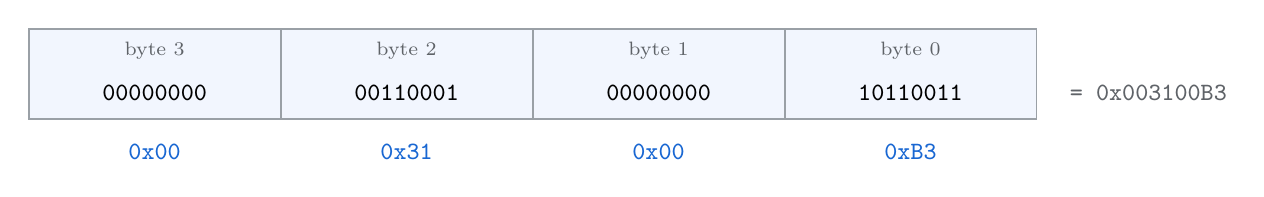
\begin{tikzpicture}[x=1cm,y=1cm]
  \newcommand{\bit}{0.40}
  \foreach \name/\val/\hex/\s in {{byte 3}/00000000/0x00/0, {byte 2}/00110001/0x31/8,
                                  {byte 1}/00000000/0x00/16, {byte 0}/10110011/0xB3/24} {
    \draw[fill=gblue!7, draw=gray5, line width=0.7pt]
      ({\s*\bit},0) rectangle ({(\s+8)*\bit},1.15);
    \node[font=\scriptsize\color{gray7}] at ({(\s+4)*\bit},0.87) {\name};
    \node[font=\small\ttfamily\bfseries] at ({(\s+4)*\bit},0.33) {\val};
    \node[font=\small\ttfamily\color{blue700}] at ({(\s+4)*\bit},-0.42) {\hex};
  }
  \node[font=\small\ttfamily\color{gray7}, anchor=west] at (13.1,0.33) {= 0x003100B3};
\end{tikzpicture}

\subsection*{how_the_cpu_reads_instructions_5}
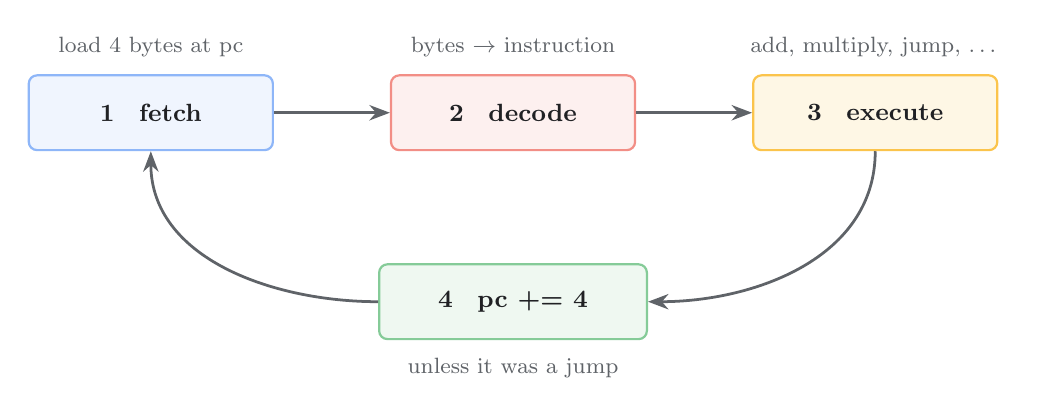
\begin{tikzpicture}[x=1cm,y=1cm]
  \node[cyclenode, fill=gblue!8, draw=gblue!60] (f) at (0,1.5) {1 \, fetch};
  \node[cyclenode, fill=gred!8, draw=gred!60] (d) at (4.6,1.5) {2 \, decode};
  \node[cyclenode, fill=gyellow!10, draw=gyellow!70] (e) at (9.2,1.5) {3 \, execute};
  \node[cyclenode, fill=ggreen!8, draw=ggreen!60, minimum width=3.4cm]
    (p) at (4.6,-0.9) {4 \, pc += 4};
  \node[font=\footnotesize\color{gray7}, above=1mm of f] {load 4 bytes at pc};
  \node[font=\footnotesize\color{gray7}, above=1mm of d] {bytes $\to$ instruction};
  \node[font=\footnotesize\color{gray7}, above=1mm of e] {add, multiply, jump, \ldots};
  \node[font=\footnotesize\color{gray7}, below=1mm of p] {unless it was a jump};
  \draw[flowarrow, gray7] (f) -- (d);
  \draw[flowarrow, gray7] (d) -- (e);
  \draw[flowarrow, gray7] (e.south) to[out=-90,in=0] (p.east);
  \draw[flowarrow, gray7] (p.west) to[out=180,in=-90] (f.south);
\end{tikzpicture}

\subsection*{endianness}
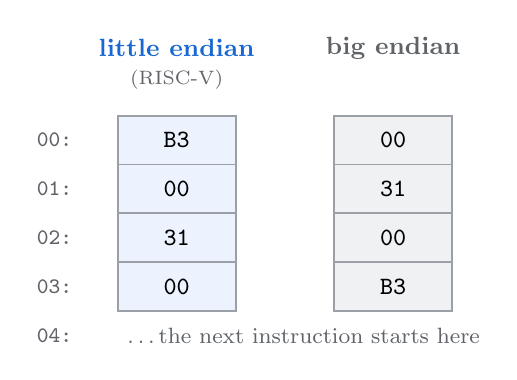
\begin{tikzpicture}[x=1cm,y=1cm,
  bcell/.style={draw=gray5, line width=0.7pt, minimum width=1.5cm,
                minimum height=0.62cm, font=\small\ttfamily}]
  \node[font=\small\bfseries\color{blue700}]  at (1.55,0.55)  {little endian};
  \node[font=\scriptsize\color{gray7}]        at (1.55,0.15)  {(RISC-V)};
  \node[font=\small\bfseries\color{gray7}]    at (4.3,0.55)   {big endian};
  \foreach \a/\le/\be/\i in {00/B3/00/1, 01/00/31/2, 02/31/00/3, 03/00/B3/4} {
    \node[addrlbl] at (0,{-\i*0.62+0.31-0.31}) {\a:};
    \node[bcell, fill=gblue!10] at (1.55,{-\i*0.62}) {\le};
    \node[bcell, fill=gray3!40] at (4.3,{-\i*0.62}) {\be};
  }
  \node[addrlbl] at (0,-3.1) {04:};
  \node[font=\footnotesize\color{gray7}, anchor=west] at (0.8,-3.1)
    {\ldots the next instruction starts here};
\end{tikzpicture}

\subsection*{arrays_and_sections}
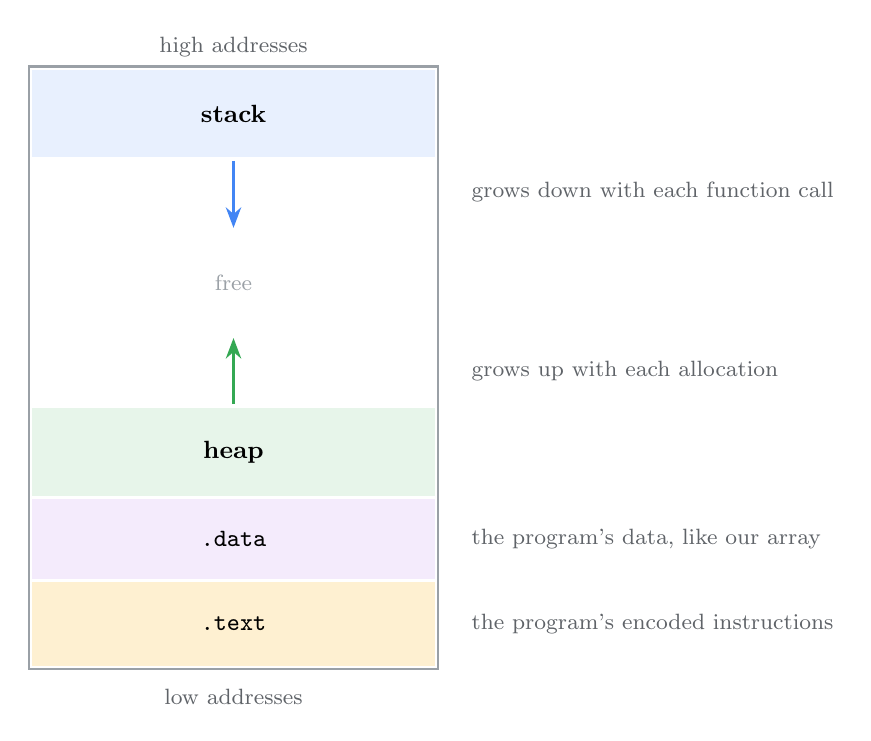
\begin{tikzpicture}[x=1cm,y=1cm]
  \node[sidelbl] at (2.6,7.9) {high addresses};
  \draw[gray5, line width=0.8pt] (0,0) rectangle (5.2,7.65);
  % stack
  \fill[gblue!12] (0.04,6.5) rectangle (5.16,7.61);
  \node[font=\small\bfseries] at (2.6,7.05) {stack};
  \draw[flowarrow, gblue] (2.6,6.45) -- (2.6,5.6);
  \node[sidelbl, anchor=west] at (5.5,6.05) {grows down with each function call};
  % heap
  \fill[ggreen!12] (0.04,2.2) rectangle (5.16,3.31);
  \node[font=\small\bfseries] at (2.6,2.75) {heap};
  \draw[flowarrow, ggreen] (2.6,3.36) -- (2.6,4.2);
  \node[sidelbl, anchor=west] at (5.5,3.78) {grows up with each allocation};
  \node[font=\footnotesize\color{gray5}] at (2.6,4.9) {free};
  % .data
  \fill[purple!10] (0.04,1.14) rectangle (5.16,2.16);
  \node[font=\small\bfseries\ttfamily] at (2.6,1.65) {.data};
  \node[sidelbl, anchor=west] at (5.5,1.65) {the program's data, like our array};
  % .text
  \fill[gyellow!18] (0.04,0.04) rectangle (5.16,1.1);
  \node[font=\small\bfseries\ttfamily] at (2.6,0.57) {.text};
  \node[sidelbl, anchor=west] at (5.5,0.57) {the program's encoded instructions};
  \node[sidelbl] at (2.6,-0.35) {low addresses};
\end{tikzpicture}

\subsection*{breakpoints_and_the_memory_view}
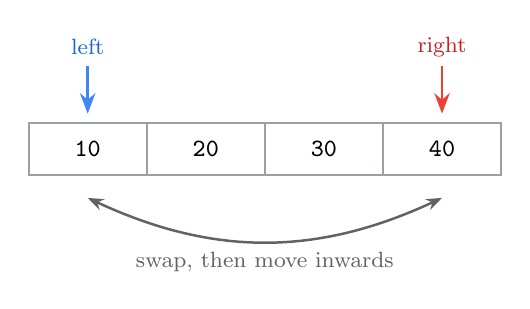
\begin{tikzpicture}[x=1cm,y=1cm,
  cell/.style={draw=gray5, line width=0.7pt, minimum width=1.5cm,
               minimum height=0.66cm, font=\small\ttfamily}]
  \foreach \v/\i in {10/0, 20/1, 30/2, 40/3}
    \node[cell, fill=white] at ({\i*1.5},0) {\v};
  \draw[flowarrow, gblue] (0,1.05) -- (0,0.45);
  \node[font=\footnotesize\color{blue700}] at (0,1.3) {left};
  \draw[flowarrow, gred] (4.5,1.05) -- (4.5,0.45);
  \node[font=\footnotesize\color{red700}] at (4.5,1.3) {right};
  \draw[{Stealth[length=2mm]}-{Stealth[length=2mm]}, gray7, line width=0.9pt]
    (0,-0.62) to[out=-25,in=205] node[below, font=\footnotesize, pos=0.5]{swap, then move inwards} (4.5,-0.62);
\end{tikzpicture}

\subsection*{functions}
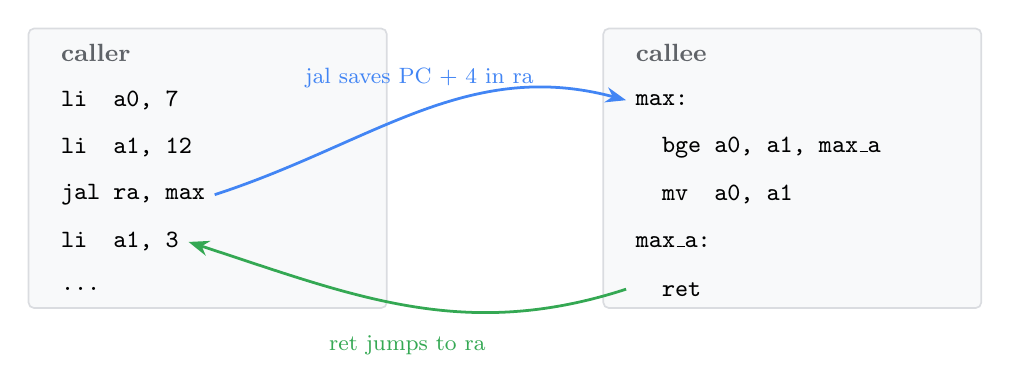
\begin{tikzpicture}[x=1cm,y=1cm,
  codeln/.style={font=\small\ttfamily, anchor=west},
  codepanel/.style={draw=gray3, fill=codebg, rounded corners=2pt, line width=0.6pt}]
  \node[codepanel, minimum width=4.55cm, minimum height=3.55cm, anchor=south west]
    at (-0.3,-0.8) {};
  \node[codepanel, minimum width=4.8cm, minimum height=3.55cm, anchor=south west]
    at (7.0,-0.8) {};
  \node[font=\small\bfseries\color{gray7}, anchor=west] at (0,2.45) {caller};
  \node[font=\small\bfseries\color{gray7}, anchor=west] at (7.3,2.45) {callee};
  % caller column
  \node[codeln] (l1) at (0,1.85) {li \ a0, 7};
  \node[codeln] (l2) at (0,1.25) {li \ a1, 12};
  \node[codeln] (l3) at (0,0.65) {jal ra, max};
  \node[codeln] (l4) at (0,0.05) {li \ a1, 3};
  \node[codeln] (l5) at (0,-0.55) {...};
  % callee column
  \node[codeln] (m0) at (7.3,1.85) {max:};
  \node[codeln] (m1) at (7.3,1.25) {\ \ bge a0, a1, max\_a};
  \node[codeln] (m2) at (7.3,0.65) {\ \ mv \ a0, a1};
  \node[codeln] (m3) at (7.3,0.05) {max\_a:};
  \node[codeln] (m4) at (7.3,-0.55) {\ \ ret};
  % arrows
  \draw[flowarrow, gblue] (l3.east) to[out=18,in=165]
    node[above=5pt, font=\footnotesize\color{blue700}, pos=0.5]{jal saves PC + 4 in ra}
    (m0.west);
  \draw[flowarrow, ggreen] (m4.west) to[out=198,in=-18]
    node[below=7pt, font=\footnotesize\color{green700}, pos=0.5]{ret jumps to ra}
    (l4.east);
\end{tikzpicture}

\subsection*{functions_2}
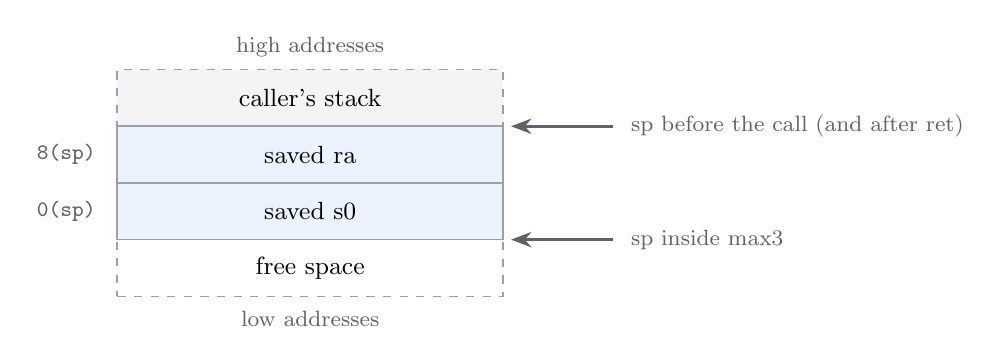
\begin{tikzpicture}[x=1cm,y=1cm]
  \node[sidelbl] at (2.45,3.4) {high addresses};
  % caller area
  \node[slot, fill=gray3!30, draw=gray5, dashed] at (2.45,2.75) {caller's stack};
  \node[slot, fill=gblue!10] (ra) at (2.45,2.03) {saved ra};
  \node[slot, fill=gblue!10] (s0) at (2.45,1.31) {saved s0};
  \node[slot, fill=white, draw=gray5, dashed] at (2.45,0.59) {free space};
  \node[addrlbl, anchor=east] at (-0.15,2.03) {8(sp)};
  \node[addrlbl, anchor=east] at (-0.15,1.31) {0(sp)};
  % sp markers
  \draw[flowarrow, gray7] (6.3,2.39) -- (5.0,2.39);
  \node[sidelbl, anchor=west] at (6.4,2.39) {sp before the call (and after ret)};
  \draw[flowarrow, gray7] (6.3,0.95) -- (5.0,0.95);
  \node[sidelbl, anchor=west] at (6.4,0.95) {sp inside max3};
  \node[sidelbl] at (2.45,-0.05) {low addresses};
\end{tikzpicture}

\subsection*{the_frame_pointer}
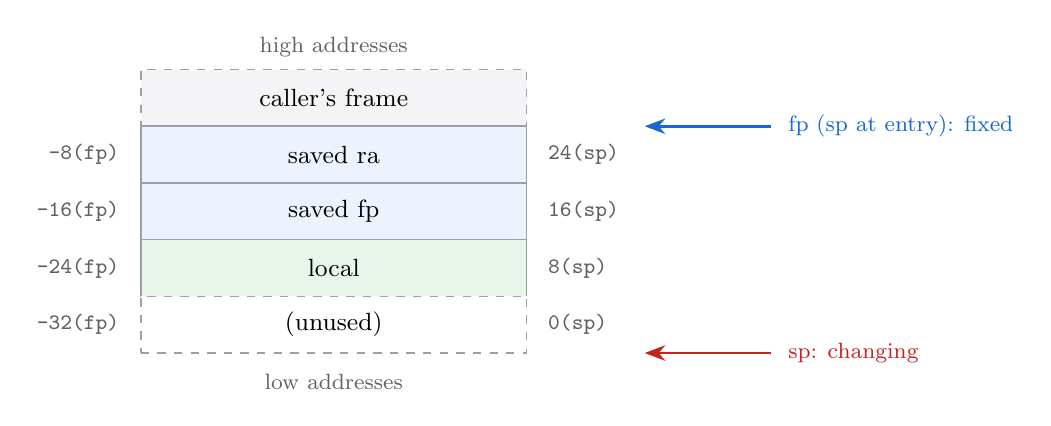
\begin{tikzpicture}[x=1cm,y=1cm]
  \node[sidelbl] at (2.45,4.15) {high addresses};
  \node[slot, fill=gray3!30, draw=gray5, dashed] at (2.45,3.5) {caller's frame};
  \node[slot, fill=gblue!10]  at (2.45,2.78) {saved ra};
  \node[slot, fill=gblue!10]  at (2.45,2.06) {saved fp};
  \node[slot, fill=ggreen!12] at (2.45,1.34) {local};
  \node[slot, fill=white, draw=gray5, dashed] at (2.45,0.62) {(unused)};
  % fp offsets left
  \node[addrlbl, anchor=east] at (-0.15,2.78) {-8(fp)};
  \node[addrlbl, anchor=east] at (-0.15,2.06) {-16(fp)};
  \node[addrlbl, anchor=east] at (-0.15,1.34) {-24(fp)};
  \node[addrlbl, anchor=east] at (-0.15,0.62) {-32(fp)};
  % sp offsets right
  \node[addrlbl, anchor=west] at (5.05,2.78) {24(sp)};
  \node[addrlbl, anchor=west] at (5.05,2.06) {16(sp)};
  \node[addrlbl, anchor=west] at (5.05,1.34) {8(sp)};
  \node[addrlbl, anchor=west] at (5.05,0.62) {0(sp)};
  % markers
  \draw[flowarrow, blue700] (8.0,3.14) -- (6.4,3.14);
  \node[sidelbl, anchor=west, color=blue700] at (8.1,3.14) {fp (sp at entry): fixed};
  \draw[flowarrow, red700] (8.0,0.26) -- (6.4,0.26);
  \node[sidelbl, anchor=west, color=red700] at (8.1,0.26) {sp: changing};
  \node[sidelbl] at (2.45,-0.1) {low addresses};
\end{tikzpicture}

\subsection*{the_frame_pointer_2}
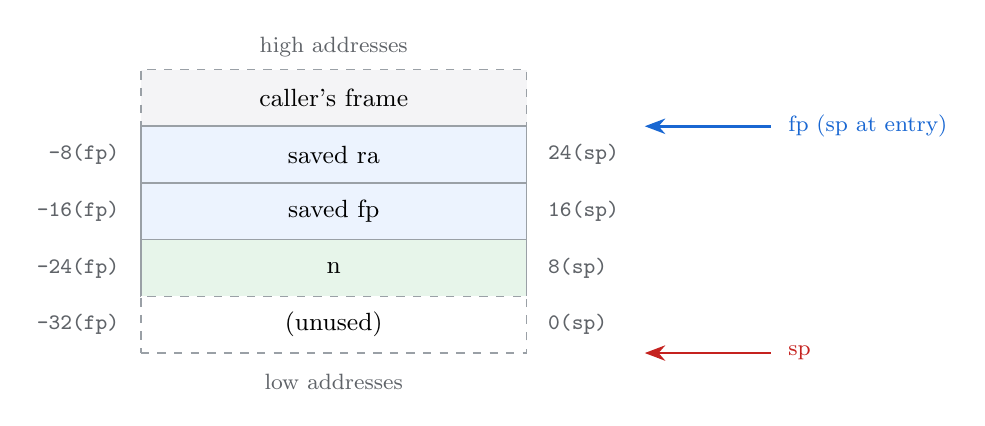
\begin{tikzpicture}[x=1cm,y=1cm]
  \node[sidelbl] at (2.45,4.15) {high addresses};
  \node[slot, fill=gray3!30, draw=gray5, dashed] at (2.45,3.5) {caller's frame};
  \node[slot, fill=gblue!10]  at (2.45,2.78) {saved ra};
  \node[slot, fill=gblue!10]  at (2.45,2.06) {saved fp};
  \node[slot, fill=ggreen!12] at (2.45,1.34) {n};
  \node[slot, fill=white, draw=gray5, dashed] at (2.45,0.62) {(unused)};
  \node[addrlbl, anchor=east] at (-0.15,2.78) {-8(fp)};
  \node[addrlbl, anchor=east] at (-0.15,2.06) {-16(fp)};
  \node[addrlbl, anchor=east] at (-0.15,1.34) {-24(fp)};
  \node[addrlbl, anchor=east] at (-0.15,0.62) {-32(fp)};
  \node[addrlbl, anchor=west] at (5.05,2.78) {24(sp)};
  \node[addrlbl, anchor=west] at (5.05,2.06) {16(sp)};
  \node[addrlbl, anchor=west] at (5.05,1.34) {8(sp)};
  \node[addrlbl, anchor=west] at (5.05,0.62) {0(sp)};
  \draw[flowarrow, blue700] (8.0,3.14) -- (6.4,3.14);
  \node[sidelbl, anchor=west, color=blue700] at (8.1,3.14) {fp (sp at entry)};
  \draw[flowarrow, red700] (8.0,0.26) -- (6.4,0.26);
  \node[sidelbl, anchor=west, color=red700] at (8.1,0.26) {sp};
  \node[sidelbl] at (2.45,-0.1) {low addresses};
\end{tikzpicture}

\subsection*{the_frame_pointer_3}
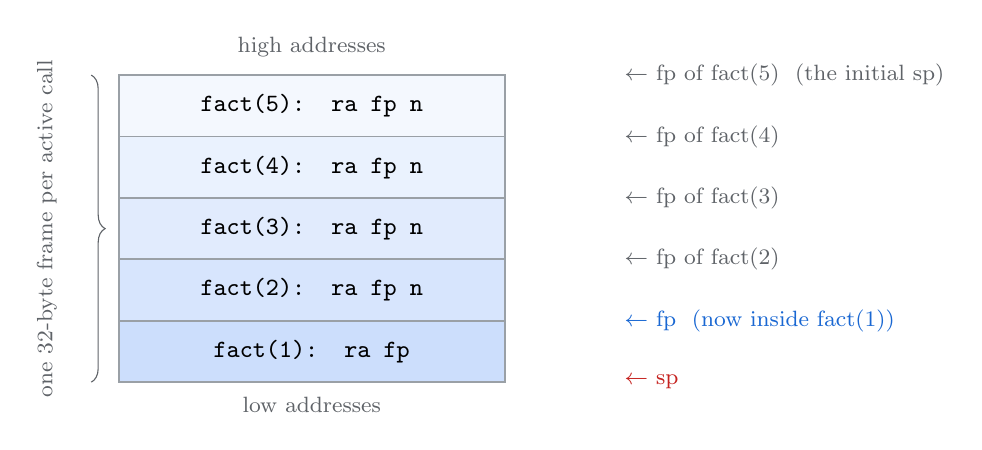
\begin{tikzpicture}[x=1cm,y=1cm,
  frame/.style={draw=gray5, line width=0.7pt, minimum width=4.9cm,
                minimum height=0.78cm, font=\small\ttfamily}]
  \node[frame, fill=gblue!6]  (f5) at (2.45,3.9)  {fact(5): ra fp n};
  \node[frame, fill=gblue!11] (f4) at (2.45,3.12) {fact(4): ra fp n};
  \node[frame, fill=gblue!16] (f3) at (2.45,2.34) {fact(3): ra fp n};
  \node[frame, fill=gblue!21] (f2) at (2.45,1.56) {fact(2): ra fp n};
  \node[frame, fill=gblue!27] (f1) at (2.45,0.78) {fact(1): ra fp};
  \node[sidelbl] at (2.45,4.65) {high addresses};
  \node[sidelbl] at (2.45,0.1)  {low addresses};
  % markers
  \node[sidelbl, anchor=west] at (6.3,4.29) {$\leftarrow$ fp of fact(5) \ (the initial sp)};
  \node[sidelbl, anchor=west] at (6.3,3.51) {$\leftarrow$ fp of fact(4)};
  \node[sidelbl, anchor=west] at (6.3,2.73) {$\leftarrow$ fp of fact(3)};
  \node[sidelbl, anchor=west] at (6.3,1.95) {$\leftarrow$ fp of fact(2)};
  \node[sidelbl, anchor=west, color=blue700] at (6.3,1.17) {$\leftarrow$ fp \ (now inside fact(1))};
  \node[sidelbl, anchor=west, color=red700]  at (6.3,0.39) {$\leftarrow$ sp};
  % depth brace
  \draw[decorate, decoration={brace, amplitude=5pt}, gray7]
    (-0.35,4.29) -- (-0.35,0.39)
    node[midway, xshift=-9pt, rotate=90, font=\footnotesize\color{gray7}, anchor=south]
    {one 32-byte frame per active call};
\end{tikzpicture}

\subsection*{the_frame_pointer_4}
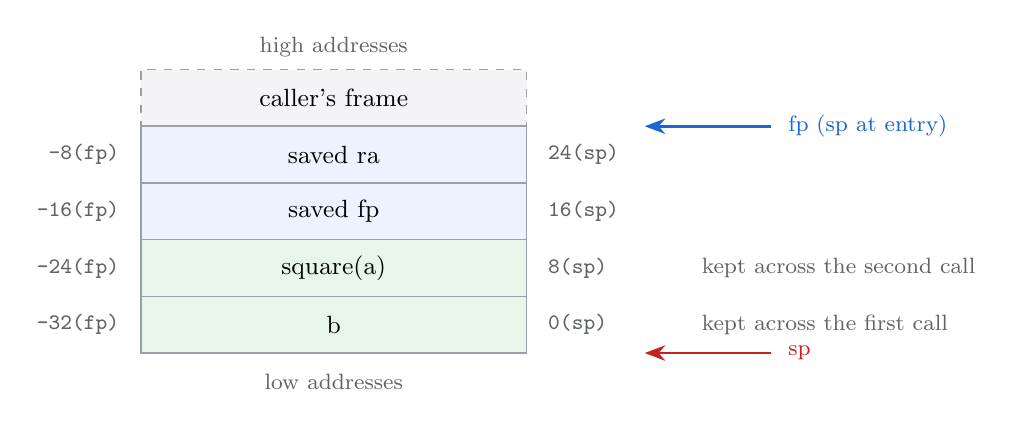
\begin{tikzpicture}[x=1cm,y=1cm]
  \node[sidelbl] at (2.45,4.15) {high addresses};
  \node[slot, fill=gray3!30, draw=gray5, dashed] at (2.45,3.5) {caller's frame};
  \node[slot, fill=gblue!10]  at (2.45,2.78) {saved ra};
  \node[slot, fill=gblue!10]  at (2.45,2.06) {saved fp};
  \node[slot, fill=ggreen!12] at (2.45,1.34) {square(a)};
  \node[slot, fill=ggreen!12] at (2.45,0.62) {b};
  \node[addrlbl, anchor=east] at (-0.15,2.78) {-8(fp)};
  \node[addrlbl, anchor=east] at (-0.15,2.06) {-16(fp)};
  \node[addrlbl, anchor=east] at (-0.15,1.34) {-24(fp)};
  \node[addrlbl, anchor=east] at (-0.15,0.62) {-32(fp)};
  \node[addrlbl, anchor=west] at (5.05,2.78) {24(sp)};
  \node[addrlbl, anchor=west] at (5.05,2.06) {16(sp)};
  \node[addrlbl, anchor=west] at (5.05,1.34) {8(sp)};
  \node[addrlbl, anchor=west] at (5.05,0.62) {0(sp)};
  \node[sidelbl, anchor=west] at (7.0,1.34) {kept across the second call};
  \node[sidelbl, anchor=west] at (7.0,0.62) {kept across the first call};
  \draw[flowarrow, blue700] (8.0,3.14) -- (6.4,3.14);
  \node[sidelbl, anchor=west, color=blue700] at (8.1,3.14) {fp (sp at entry)};
  \draw[flowarrow, red700] (8.0,0.26) -- (6.4,0.26);
  \node[sidelbl, anchor=west, color=red700] at (8.1,0.26) {sp};
  \node[sidelbl] at (2.45,-0.1) {low addresses};
\end{tikzpicture}

\subsection*{bit_representations}
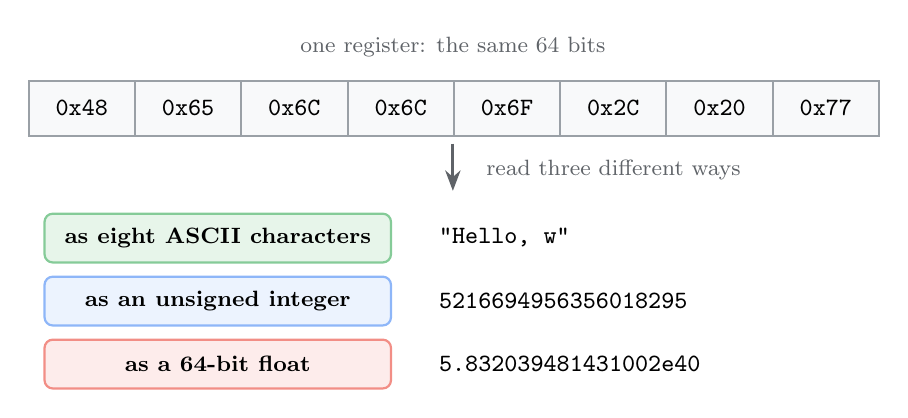
\begin{tikzpicture}[x=1cm,y=1cm,
  bytecell/.style={draw=gray5, line width=0.7pt, fill=codebg, minimum width=1.35cm,
                   minimum height=0.7cm, font=\small\ttfamily, anchor=west},
  chip/.style={rounded corners=3pt, line width=0.8pt, minimum width=4.4cm,
               minimum height=0.62cm, font=\footnotesize\bfseries, anchor=west},
  val/.style={font=\small\ttfamily, anchor=west}]
  % one register holding eight bytes
  \node[font=\footnotesize\color{gray7}] at (5.4,0.78) {one register: the same 64 bits};
  \foreach \v/\i in {0x48/0, 0x65/1, 0x6C/2, 0x6C/3, 0x6F/4, 0x2C/5, 0x20/6, 0x77/7}
    \node[bytecell] at ({\i*1.35},0) {\v};
  % three readings of those bits
  \draw[flowarrow, gray7] (5.4,-0.45) -- (5.4,-1.05);
  \node[font=\footnotesize\color{gray7}, anchor=west] at (5.7,-0.78) {read three different ways};
  \node[chip, fill=ggreen!12, draw=ggreen!60] at (0.2,-1.65) {as eight ASCII characters};
  \node[chip, fill=gblue!10,  draw=gblue!60]  at (0.2,-2.45) {as an unsigned integer};
  \node[chip, fill=gred!10,   draw=gred!60]   at (0.2,-3.25) {as a 64-bit float};
  \node[val] at (5.1,-1.65) {"Hello, w"};
  \node[val] at (5.1,-2.45) {5216694956356018295};
  \node[val] at (5.1,-3.25) {5.832039481431002e40};
\end{tikzpicture}

\subsection*{an_address_is_also_just_a_number}
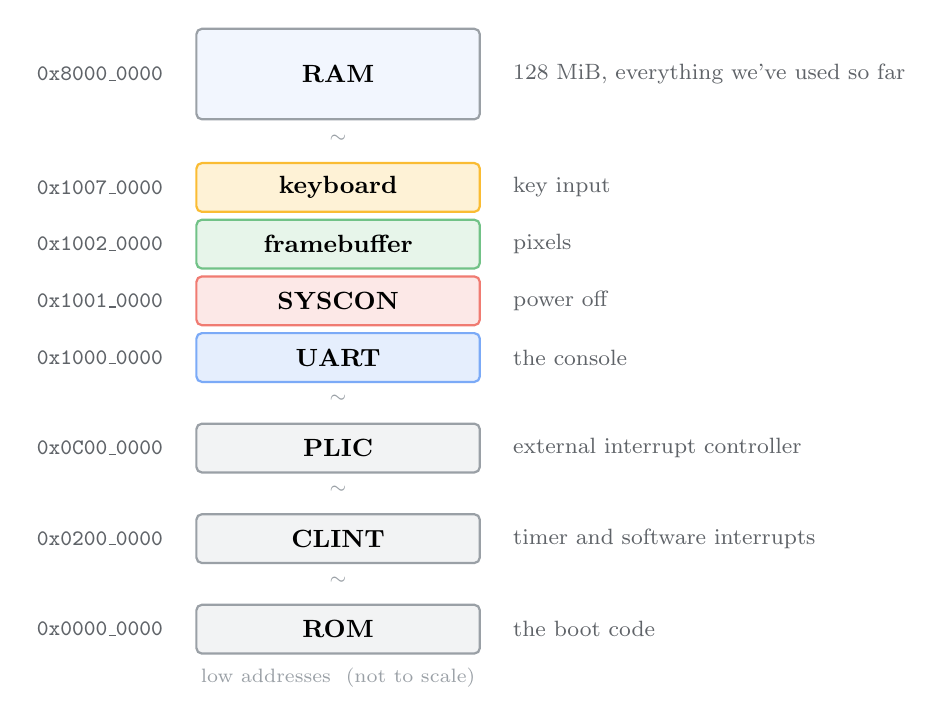
\begin{tikzpicture}[x=1cm,y=1cm,
  dev/.style={draw, line width=0.8pt, rounded corners=2pt, minimum width=3.6cm,
              minimum height=0.62cm, font=\small\bfseries},
  gap/.style={font=\scriptsize\color{gray5}}]
  % from bottom (low addresses) to top
  \node[dev, fill=gray3!35, draw=gray5]      (rom)  at (0,0)    {ROM};
  \node[gap] at (0,0.62) {$\sim$};
  \node[dev, fill=gray3!35, draw=gray5]      (cl)   at (0,1.15) {CLINT};
  \node[gap] at (0,1.77) {$\sim$};
  \node[dev, fill=gray3!35, draw=gray5]      (pl)   at (0,2.3)  {PLIC};
  \node[gap] at (0,2.92) {$\sim$};
  \node[dev, fill=gblue!14, draw=gblue!70]   (ua)   at (0,3.45) {UART};
  \node[dev, fill=gred!12, draw=gred!70]     (sc)   at (0,4.17) {SYSCON};
  \node[dev, fill=ggreen!12, draw=ggreen!70] (fb)   at (0,4.89) {framebuffer};
  \node[dev, fill=gyellow!16, draw=gyellow!80] (kb) at (0,5.61) {keyboard};
  \node[gap] at (0,6.23) {$\sim$};
  \node[dev, fill=gblue!7, draw=gray5, minimum height=1.15cm] (ram) at (0,7.05) {RAM};
  % addresses left
  \node[addrlbl, anchor=east] at (-2.1,0)    {0x0000\_0000};
  \node[addrlbl, anchor=east] at (-2.1,1.15) {0x0200\_0000};
  \node[addrlbl, anchor=east] at (-2.1,2.3)  {0x0C00\_0000};
  \node[addrlbl, anchor=east] at (-2.1,3.45) {0x1000\_0000};
  \node[addrlbl, anchor=east] at (-2.1,4.17) {0x1001\_0000};
  \node[addrlbl, anchor=east] at (-2.1,4.89) {0x1002\_0000};
  \node[addrlbl, anchor=east] at (-2.1,5.61) {0x1007\_0000};
  \node[addrlbl, anchor=east] at (-2.1,7.05) {0x8000\_0000};
  % descriptions right
  \node[sidelbl, anchor=west] at (2.1,0)    {the boot code};
  \node[sidelbl, anchor=west] at (2.1,1.15) {timer and software interrupts};
  \node[sidelbl, anchor=west] at (2.1,2.3)  {external interrupt controller};
  \node[sidelbl, anchor=west] at (2.1,3.45) {the console};
  \node[sidelbl, anchor=west] at (2.1,4.17) {power off};
  \node[sidelbl, anchor=west] at (2.1,4.89) {pixels};
  \node[sidelbl, anchor=west] at (2.1,5.61) {key input};
  \node[sidelbl, anchor=west] at (2.1,7.05) {128 MiB, everything we've used so far};
  \node[font=\scriptsize\color{gray5}] at (0,-0.62) {low addresses \ (not to scale)};
\end{tikzpicture}

\subsection*{uart}
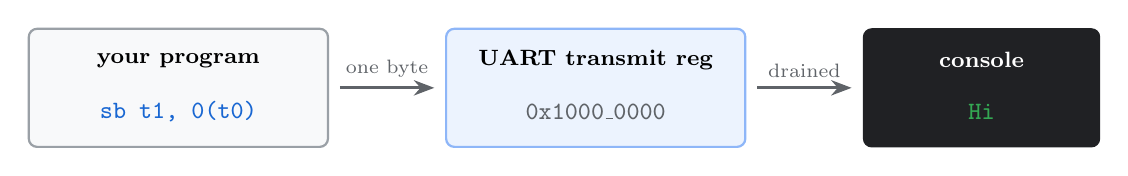
\begin{tikzpicture}[x=1cm,y=1cm]
  \draw[rounded corners=3pt, fill=codebg, draw=gray5, line width=0.8pt]
    (0,0) rectangle (3.8,1.5);
  \node[font=\footnotesize\bfseries] at (1.9,1.1) {your program};
  \node[font=\small\ttfamily\color{blue700}] at (1.9,0.45) {sb t1, 0(t0)};
  \draw[rounded corners=3pt, fill=gblue!10, draw=gblue!60, line width=0.8pt]
    (5.3,0) rectangle (9.1,1.5);
  \node[font=\footnotesize\bfseries] at (7.2,1.1) {UART transmit reg};
  \node[font=\small\ttfamily\color{gray7}] at (7.2,0.45) {0x1000\_0000};
  \draw[rounded corners=3pt, fill=ink, draw=ink]
    (10.6,0) rectangle (13.6,1.5);
  \node[font=\footnotesize\bfseries\color{white}] at (12.1,1.1) {console};
  \node[font=\small\ttfamily\color{ggreen}] at (12.1,0.45) {Hi};
  \draw[flowarrow, gray7] (3.95,0.75) -- node[above,font=\scriptsize]{one byte} (5.15,0.75);
  \draw[flowarrow, gray7] (9.25,0.75) -- node[above,font=\scriptsize]{drained} (10.45,0.75);
\end{tikzpicture}

\subsection*{the_power_off_device}

\begin{tikzpicture}[x=1cm,y=1cm]
  \newcommand{\bit}{0.40}
  % I-type: imm[11:0] (12) rs1 (5) funct3 (3) rd (5) opcode (7)
  \foreach \name/\s/\w/\col in {{imm[11:0]}/0/12/gyellow, rs1/12/5/gred,
                                 funct3/17/3/gray5, rd/20/5/gblue, opcode/25/7/ggreen} {
    \draw[fill=\col!14, draw=\col!70!black!60, line width=0.7pt]
      ({\s*\bit},0) rectangle ({(\s+\w)*\bit},0.85);
    \node[font=\small\ttfamily] at ({(\s+\w/2)*\bit},0.425) {\name};
  }
\end{tikzpicture}

\subsection*{the_linker_script}
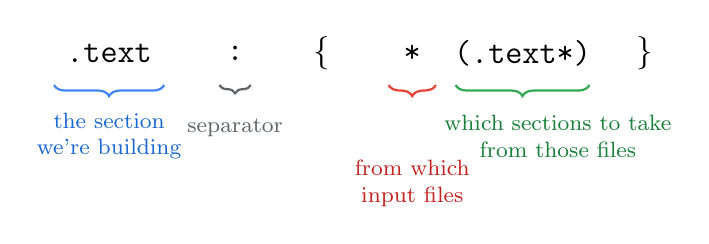
\begin{tikzpicture}[x=1cm,y=1cm]
  \node[font=\large\ttfamily] (a) at (0.7,0)  {.text};
  \node[font=\large\ttfamily] (b) at (2.3,0)  {:};
  \node[font=\large\ttfamily] (c) at (3.4,0)  {\{};
  \node[font=\large\ttfamily] (d) at (4.55,0) {*};
  \node[font=\large\ttfamily] (e) at (5.95,0) {(.text*)};
  \node[font=\large\ttfamily] (f) at (7.5,0)  {\}};
  % braces + labels
  \draw[decorate, decoration={brace, mirror, amplitude=4pt}, gblue, line width=0.8pt]
    (0.0,-0.4) -- (1.4,-0.4);
  \node[font=\footnotesize\color{blue700}, align=center] at (0.7,-1.05)
    {the section\\we're building};
  \draw[decorate, decoration={brace, mirror, amplitude=3pt}, gray7, line width=0.8pt]
    (2.1,-0.4) -- (2.5,-0.4);
  \node[font=\footnotesize\color{gray7}] at (2.3,-0.95) {separator};
  \draw[decorate, decoration={brace, mirror, amplitude=4pt}, gred, line width=0.8pt]
    (4.25,-0.4) -- (4.85,-0.4);
  \node[font=\footnotesize\color{red700}, align=center] at (4.55,-1.65)
    {from which\\input files};
  \draw[decorate, decoration={brace, mirror, amplitude=4pt}, ggreen, line width=0.8pt]
    (5.1,-0.4) -- (6.8,-0.4);
  \node[font=\footnotesize\color{green700}, align=center] at (6.4,-1.05)
    {which sections to take\\from those files};
\end{tikzpicture}

\subsection*{the_linker_script_2}
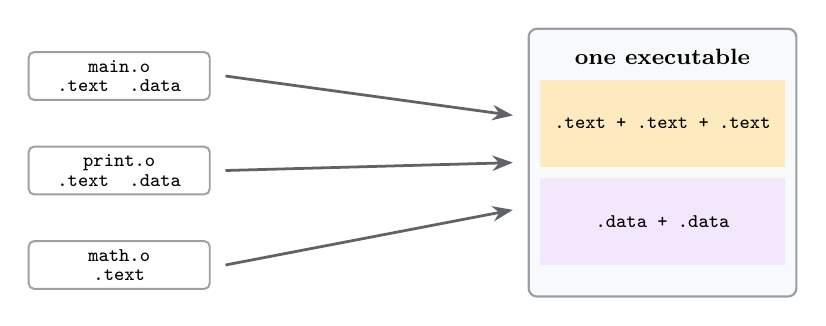
\begin{tikzpicture}[x=1cm,y=1cm,
  objf/.style={draw=gray5, line width=0.7pt, rounded corners=2pt, minimum width=2.3cm,
               font=\scriptsize\ttfamily, align=center, inner sep=3pt}]
  % input files
  \node[objf, fill=white] (f1) at (0,2.4) {main.o\\[-1pt] .text \ .data};
  \node[objf, fill=white] (f2) at (0,1.2) {print.o\\[-1pt] .text \ .data};
  \node[objf, fill=white] (f3) at (0,0.0) {math.o\\[-1pt] .text};
  % output
  \draw[rounded corners=3pt, fill=codebg, draw=gray5, line width=0.8pt]
    (5.2,-0.4) rectangle (8.6,3.0);
  \node[font=\footnotesize\bfseries] at (6.9,2.65) {one executable};
  \fill[gyellow!25] (5.35,1.25) rectangle (8.45,2.35);
  \node[font=\scriptsize\ttfamily] at (6.9,1.8) {.text + .text + .text};
  \fill[purple!12] (5.35,0.0) rectangle (8.45,1.1);
  \node[font=\scriptsize\ttfamily] at (6.9,0.55) {.data + .data};
  % arrows
  \draw[flowarrow, gray7] (1.35,2.4) -- (5.0,1.9);
  \draw[flowarrow, gray7] (1.35,1.2) -- (5.0,1.3);
  \draw[flowarrow, gray7] (1.35,0.0) -- (5.0,0.7);
\end{tikzpicture}

\subsection*{how_real_is_real_enough}
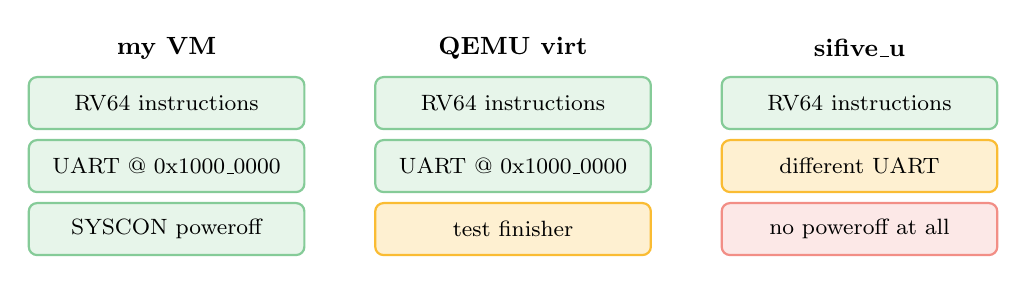
\begin{tikzpicture}[x=1cm,y=1cm,
  mach/.style={rounded corners=3pt, line width=0.8pt, minimum width=3.5cm,
               minimum height=0.66cm, font=\footnotesize}]
  \node[font=\small\bfseries] at (2.0,3.4)  {my VM};
  \node[font=\small\bfseries] at (6.4,3.4)  {QEMU virt};
  \node[font=\small\bfseries] at (10.8,3.4) {sifive\_u};
  % instructions row: portable
  \foreach \x in {2.0,6.4,10.8}
    \node[mach, fill=ggreen!12, draw=ggreen!60] at (\x,2.7) {RV64 instructions};
  % uart row
  \node[mach, fill=ggreen!12, draw=ggreen!60] at (2.0,1.9)  {UART @ 0x1000\_0000};
  \node[mach, fill=ggreen!12, draw=ggreen!60] at (6.4,1.9)  {UART @ 0x1000\_0000};
  \node[mach, fill=gyellow!18, draw=gyellow!80] at (10.8,1.9) {different UART};
  % poweroff row
  \node[mach, fill=ggreen!12, draw=ggreen!60] at (2.0,1.1)  {SYSCON poweroff};
  \node[mach, fill=gyellow!18, draw=gyellow!80] at (6.4,1.1) {test finisher};
  \node[mach, fill=gred!12, draw=gred!60] at (10.8,1.1)     {no poweroff at all};
\end{tikzpicture}

\subsection*{compilers_and_ir}
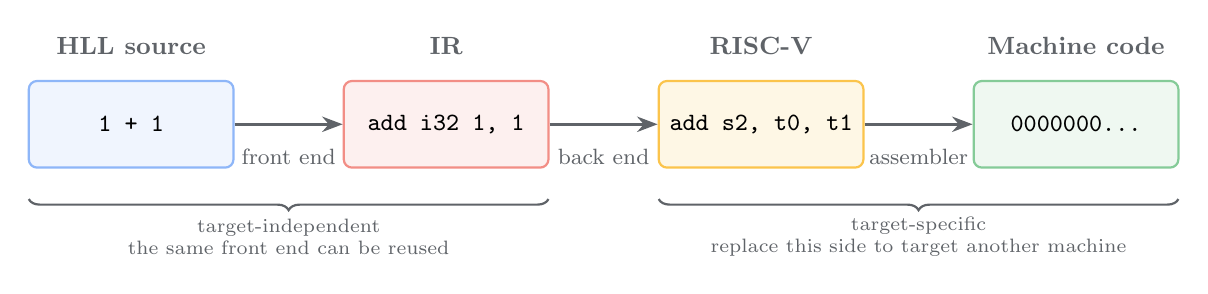
\begin{tikzpicture}[
  stage/.style={rounded corners=3pt, line width=0.8pt, minimum width=2.6cm,
                minimum height=1.1cm, align=center},
  heading/.style={font=\small\bfseries\color{gray7}},
  code/.style={font=\small\ttfamily},
  label/.style={font=\footnotesize\color{gray7}},
  note/.style={font=\scriptsize\color{gray7}, align=center}]
  \node[heading] at (0,1.0) {HLL source};
  \node[heading] at (4.0,1.0) {IR};
  \node[heading] at (8.0,1.0) {RISC-V};
  \node[heading] at (12.0,1.0) {Machine code};

  \node[stage, fill=gblue!8, draw=gblue!60] (hll) at (0,0)
    {\small\ttfamily 1 + 1};
  \node[stage, fill=gred!8, draw=gred!60] (ir) at (4.0,0)
    {\small\ttfamily add i32 1, 1};
  \node[stage, fill=gyellow!10, draw=gyellow!70] (asm) at (8.0,0)
    {\small\ttfamily add s2, t0, t1};
  \node[stage, fill=ggreen!8, draw=ggreen!60] (bits) at (12.0,0)
    {\small\ttfamily 0000000\ldots};

  \draw[flowarrow, gray7] (hll) -- node[below=5pt, label] {front end} (ir);
  \draw[flowarrow, gray7] (ir) -- node[below=5pt, label] {back end} (asm);
  \draw[flowarrow, gray7] (asm) -- node[below=5pt, label] {assembler} (bits);

  \draw[decorate, decoration={brace, mirror, amplitude=4pt}, gray7,
        line width=0.8pt] (-1.3,-0.95) -- (5.3,-0.95);
  \node[note] at (2.0,-1.43)
    {target-independent\\the same front end can be reused};
  \draw[decorate, decoration={brace, mirror, amplitude=4pt}, gray7,
        line width=0.8pt] (6.7,-0.95) -- (13.3,-0.95);
  \node[note] at (10.0,-1.43)
    {target-specific\\replace this side to target another machine};
\end{tikzpicture}

\subsection*{from_hll_to_an_executable}
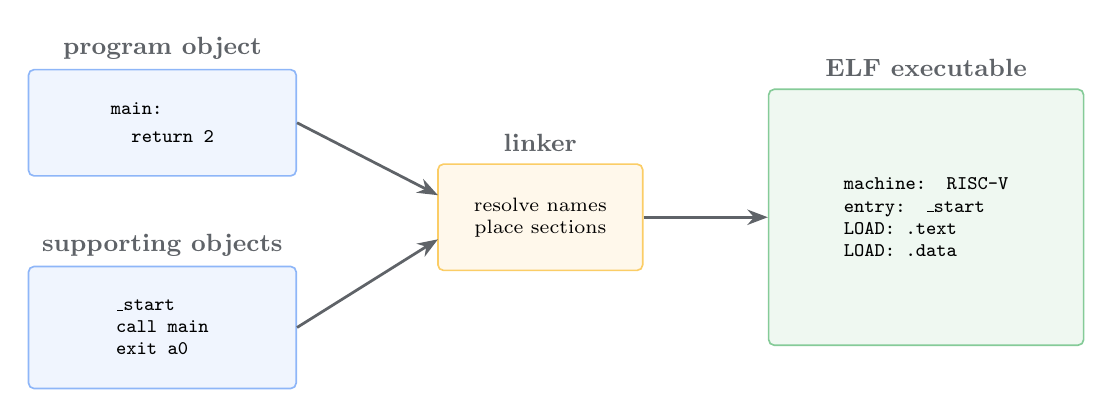
\begin{tikzpicture}[
  panel/.style={draw=gray3, fill=codebg, rounded corners=2pt, line width=0.6pt,
                align=left},
  heading/.style={font=\small\bfseries\color{gray7}},
  code/.style={font=\scriptsize\ttfamily, align=left}]
  \node[heading] at (0,2.25) {program object};
  \node[panel, fill=gblue!8, draw=gblue!60, minimum width=3.4cm,
        minimum height=1.35cm] (user) at (0,1.3) {};
  \node[code] at (0,1.3) {main:\\[2pt]\ \ return 2};

  \node[heading] at (0,-0.25) {supporting objects};
  \node[panel, fill=gblue!8, draw=gblue!60, minimum width=3.4cm,
        minimum height=1.55cm] (support) at (0,-1.3) {};
  \node[code] at (0,-1.3) {\_start\\call main\\exit a0};

  \node[heading] at (4.8,1.05) {linker};
  \node[panel, fill=gyellow!8, draw=gyellow!60, minimum width=2.6cm,
        minimum height=1.35cm] (linker) at (4.8,0.1) {};
  \node[font=\scriptsize, align=center] at (4.8,0.1)
    {resolve names\\place sections};

  \node[heading] at (9.7,2.0) {ELF executable};
  \node[panel, fill=ggreen!8, draw=ggreen!60, minimum width=4.0cm,
        minimum height=3.25cm] (elf) at (9.7,0.1) {};
  \node[code] at (9.7,0.1) {machine: RISC-V\\entry: \_start\\LOAD: .text\\LOAD: .data};

  \draw[flowarrow, gray7] (user.east) -- (3.5,0.38);
  \draw[flowarrow, gray7] (support.east) -- (3.5,-0.18);
  \draw[flowarrow, gray7] (linker.east) -- (elf.west);
\end{tikzpicture}

\subsection*{watching_it_run}
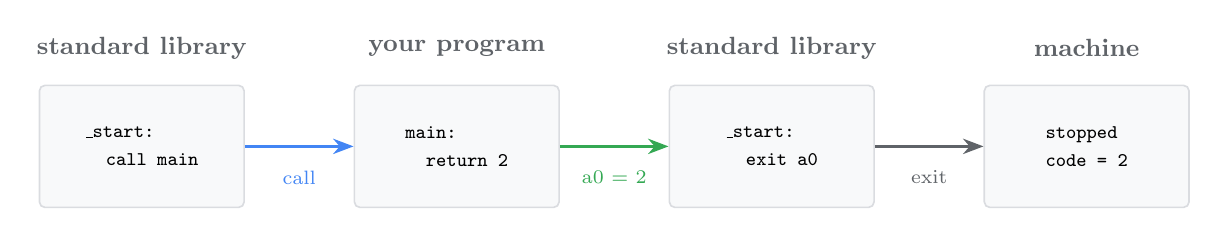
\begin{tikzpicture}[
  stage/.style={draw=gray3, fill=codebg, rounded corners=2pt, line width=0.6pt,
                minimum width=2.6cm, minimum height=1.55cm, align=left},
  heading/.style={font=\small\bfseries\color{gray7}},
  code/.style={font=\scriptsize\ttfamily, align=left}]
  \node[heading] at (0,1.25) {standard library};
  \node[heading] at (4,1.25) {your program};
  \node[heading] at (8,1.25) {standard library};
  \node[heading] at (12,1.25) {machine};

  \node[stage] (start) at (0,0) {};
  \node[code] at (0,0) {\_start:\\[2pt]\ \ call main};
  \node[stage] (main) at (4,0) {};
  \node[code] at (4,0) {main:\\[2pt]\ \ return 2};
  \node[stage] (return) at (8,0) {};
  \node[code] at (8,0) {\_start:\\[2pt]\ \ exit a0};
  \node[stage] (stop) at (12,0) {};
  \node[code] at (12,0) {stopped\\[2pt]code = 2};

  \draw[flowarrow, gblue] (start) --
    node[below=5pt, font=\scriptsize\color{blue700}] {call} (main);
  \draw[flowarrow, ggreen] (main) --
    node[below=5pt, font=\scriptsize\color{green700}] {a0 = 2} (return);
  \draw[flowarrow, gray7] (return) --
    node[below=5pt, font=\scriptsize\color{gray7}] {exit} (stop);
\end{tikzpicture}

\subsection*{exit_function}
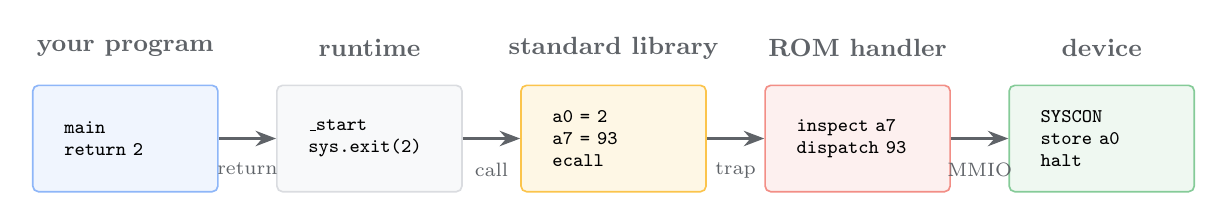
\begin{tikzpicture}[
  stage/.style={draw=gray3, fill=codebg, rounded corners=2pt, line width=0.6pt,
                minimum width=2.35cm, minimum height=1.35cm, align=center},
  heading/.style={font=\small\bfseries\color{gray7}},
  code/.style={font=\scriptsize\ttfamily, align=left, text width=1.55cm},
  edge/.style={flowarrow, gray7},
  edge label/.style={font=\scriptsize\color{gray7}, align=center}]
  \node[heading] at (0,1.15) {your program};
  \node[heading] at (3.1,1.15) {runtime};
  \node[heading] at (6.2,1.15) {standard library};
  \node[heading] at (9.3,1.15) {ROM handler};
  \node[heading] at (12.4,1.15) {device};

  \node[stage, fill=gblue!8, draw=gblue!60] (main) at (0,0) {};
  \node[code] at (0,0) {main\\return 2};
  \node[stage] (runtime) at (3.1,0) {};
  \node[code] at (3.1,0) {\_start\\sys.exit(2)};
  \node[stage, fill=gyellow!10, draw=gyellow!70] (wrapper) at (6.2,0) {};
  \node[code] at (6.2,0) {a0 = 2\\a7 = 93\\ecall};
  \node[stage, fill=gred!8, draw=gred!60] (handler) at (9.3,0) {};
  \node[code] at (9.3,0) {inspect a7\\dispatch 93};
  \node[stage, fill=ggreen!8, draw=ggreen!60] (syscon) at (12.4,0) {};
  \node[code] at (12.4,0) {SYSCON\\store a0\\halt};

  \draw[edge] (main) -- node[below=5pt, edge label] {return} (runtime);
  \draw[edge] (runtime) -- node[below=5pt, edge label] {call} (wrapper);
  \draw[edge] (wrapper) -- node[below=5pt, edge label] {trap} (handler);
  \draw[edge] (handler) -- node[below=5pt, edge label] {MMIO} (syscon);
\end{tikzpicture}

\subsection*{why_abstract_it}
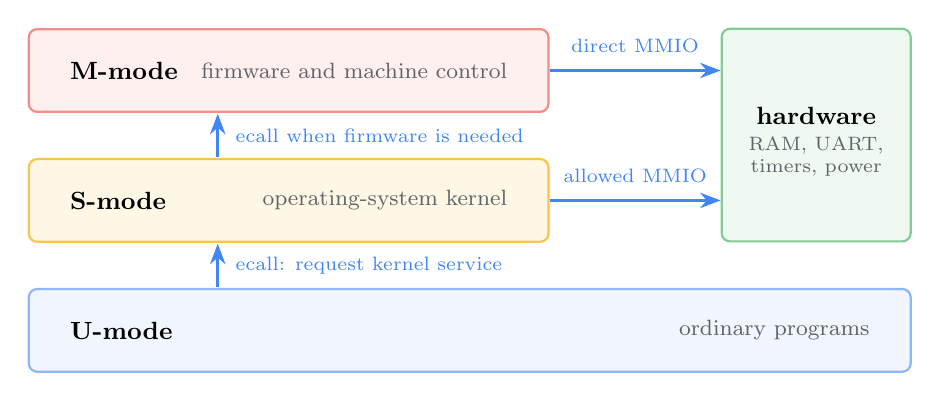
\begin{tikzpicture}[
  layer/.style={rounded corners=3pt, line width=0.8pt, minimum width=6.6cm,
                minimum height=1.05cm},
  title/.style={font=\small\bfseries, anchor=west},
  detail/.style={font=\footnotesize\color{gray7}, anchor=east},
  request/.style={-{Stealth[length=2.6mm]}, line width=1pt, gblue},
  request label/.style={font=\scriptsize\color{blue700}, fill=none, inner sep=2pt}]
  \node[layer, minimum width=11.2cm, fill=gblue!8, draw=gblue!60] (user) at (0,0) {};
  \node[title] at (-5.2,0) {U-mode};
  \node[detail] at (5.2,0) {ordinary programs};

  \node[layer, fill=gyellow!10, draw=gyellow!70] (supervisor) at (-2.3,1.65) {};
  \node[title] at (-5.2,1.65) {S-mode};
  \node[detail] at (0.6,1.65) {operating-system kernel};

  \node[layer, fill=gred!8, draw=gred!60] (machine) at (-2.3,3.3) {};
  \node[title] at (-5.2,3.3) {M-mode};
  \node[detail] at (0.6,3.3) {firmware and machine control};

  \node[layer, minimum width=2.4cm, minimum height=2.7cm,
        fill=ggreen!8, draw=ggreen!60] (devices) at (4.4,2.48) {};
  \node[font=\small\bfseries] at (4.4,2.72) {hardware};
  \node[font=\scriptsize\color{gray7}, align=center] at (4.4,2.2)
    {RAM, UART,\\timers, power};

  \draw[request] (-3.2,0.55) --
    node[right=4pt, request label] {ecall: request kernel service} (-3.2,1.1);
  \draw[request] (-3.2,2.2) --
    node[right=4pt, request label] {ecall when firmware is needed} (-3.2,2.75);
  \draw[request] (supervisor.east) --
    node[above=4pt, request label] {allowed MMIO} (devices.west |- supervisor.east);
  \draw[request] (machine.east) --
    node[above=4pt, request label] {direct MMIO} (devices.west |- machine.east);
\end{tikzpicture}

\subsection*{dynamic_memory_allocation}
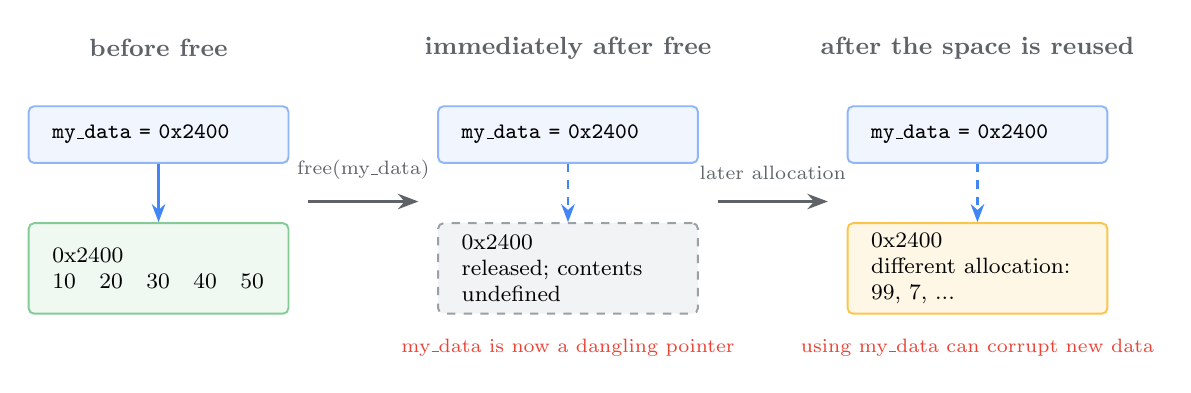
\begin{tikzpicture}[
  stage title/.style={font=\small\bfseries\color{gray7}},
  pointer/.style={rounded corners=2pt, line width=0.7pt, minimum width=3.3cm,
                  minimum height=0.72cm, align=left, font=\footnotesize\ttfamily,
                  text width=2.7cm},
  region/.style={rounded corners=2pt, line width=0.7pt, minimum width=3.3cm,
                 minimum height=1.15cm, align=left, font=\footnotesize,
                 text width=2.7cm},
  ptr/.style={-{Stealth[length=2.3mm]}, line width=0.9pt, gblue},
  transition/.style={-{Stealth[length=2.6mm]}, line width=1pt, gray7},
  note/.style={font=\scriptsize\color{gray7}, align=center}]
  \node[stage title] at (0,2.55) {before free};
  \node[pointer, fill=gblue!8, draw=gblue!60] (ptr1) at (0,1.45)
    {my\_data = 0x2400};
  \node[region, fill=ggreen!8, draw=ggreen!60] (heap1) at (0,-0.25)
    {0x2400\\10\quad 20\quad 30\quad 40\quad 50};
  \draw[ptr] (ptr1.south) -- (heap1.north);

  \node[stage title] at (5.2,2.55) {immediately after free};
  \node[pointer, fill=gblue!8, draw=gblue!60] (ptr2) at (5.2,1.45)
    {my\_data = 0x2400};
  \node[region, fill=gray3!35, draw=gray5, dashed] (heap2) at (5.2,-0.25)
    {0x2400\\released; contents undefined};
  \draw[ptr, dashed] (ptr2.south) -- (heap2.north);
  \node[note, text=gred] at (5.2,-1.25) {my\_data is now a dangling pointer};

  \node[stage title] at (10.4,2.55) {after the space is reused};
  \node[pointer, fill=gblue!8, draw=gblue!60] (ptr3) at (10.4,1.45)
    {my\_data = 0x2400};
  \node[region, fill=gyellow!10, draw=gyellow!70] (heap3) at (10.4,-0.25)
    {0x2400\\different allocation: 99, 7, ...};
  \draw[ptr, dashed] (ptr3.south) -- (heap3.north);
  \node[note, text=gred] at (10.4,-1.25) {using my\_data can corrupt new data};

  \draw[transition] (1.9,0.6) -- node[above=4pt, note] {free(my\_data)} (3.3,0.6);
  \draw[transition] (7.1,0.6) -- node[above=4pt, note] {later allocation} (8.5,0.6);
\end{tikzpicture}

\subsection*{dynamic_memory_allocation_2}
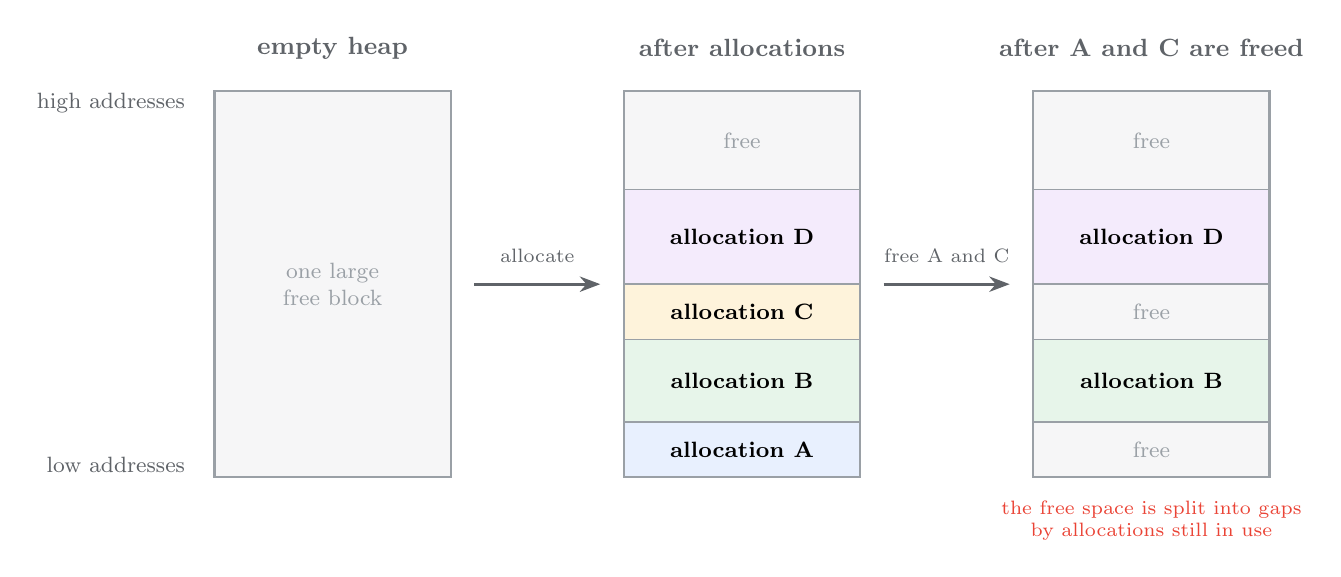
\begin{tikzpicture}[
  stage title/.style={font=\small\bfseries\color{gray7}},
  block label/.style={font=\footnotesize\bfseries, align=center},
  free label/.style={font=\footnotesize\color{gray5}, align=center},
  note/.style={font=\scriptsize\color{gray7}, align=center},
  transition/.style={-{Stealth[length=2.6mm]}, line width=1pt, gray7}]
  \node[stage title] at (0,5.45) {empty heap};
  \fill[gray3!25] (-1.5,0) rectangle (1.5,4.9);
  \draw[gray5, line width=0.8pt] (-1.5,0) rectangle (1.5,4.9);
  \node[free label] at (0,2.45) {one large\\free block};

  \node[stage title] at (5.2,5.45) {after allocations};
  \fill[gblue!12] (3.7,0) rectangle (6.7,0.7);
  \fill[ggreen!12] (3.7,0.7) rectangle (6.7,1.75);
  \fill[gyellow!14] (3.7,1.75) rectangle (6.7,2.45);
  \fill[purple!10] (3.7,2.45) rectangle (6.7,3.65);
  \fill[gray3!25] (3.7,3.65) rectangle (6.7,4.9);
  \draw[gray5, line width=0.8pt] (3.7,0) rectangle (6.7,4.9);
  \draw[gray5, line width=0.55pt] (3.7,0.7) -- (6.7,0.7);
  \draw[gray5, line width=0.55pt] (3.7,1.75) -- (6.7,1.75);
  \draw[gray5, line width=0.55pt] (3.7,2.45) -- (6.7,2.45);
  \draw[gray5, line width=0.55pt] (3.7,3.65) -- (6.7,3.65);
  \node[block label] at (5.2,0.35) {allocation A};
  \node[block label] at (5.2,1.225) {allocation B};
  \node[block label] at (5.2,2.1) {allocation C};
  \node[block label] at (5.2,3.05) {allocation D};
  \node[free label] at (5.2,4.275) {free};

  \node[stage title] at (10.4,5.45) {after A and C are freed};
  \fill[gray3!25] (8.9,0) rectangle (11.9,0.7);
  \fill[ggreen!12] (8.9,0.7) rectangle (11.9,1.75);
  \fill[gray3!25] (8.9,1.75) rectangle (11.9,2.45);
  \fill[purple!10] (8.9,2.45) rectangle (11.9,3.65);
  \fill[gray3!25] (8.9,3.65) rectangle (11.9,4.9);
  \draw[gray5, line width=0.8pt] (8.9,0) rectangle (11.9,4.9);
  \draw[gray5, line width=0.55pt] (8.9,0.7) -- (11.9,0.7);
  \draw[gray5, line width=0.55pt] (8.9,1.75) -- (11.9,1.75);
  \draw[gray5, line width=0.55pt] (8.9,2.45) -- (11.9,2.45);
  \draw[gray5, line width=0.55pt] (8.9,3.65) -- (11.9,3.65);
  \node[free label] at (10.4,0.35) {free};
  \node[block label] at (10.4,1.225) {allocation B};
  \node[free label] at (10.4,2.1) {free};
  \node[block label] at (10.4,3.05) {allocation D};
  \node[free label] at (10.4,4.275) {free};
  \node[note, text=gred] at (10.4,-0.55)
    {the free space is split into gaps\\by allocations still in use};

  \draw[transition] (1.8,2.45) -- node[above=4pt, note] {allocate} (3.4,2.45);
  \draw[transition] (7,2.45) -- node[above=4pt, note] {free A and C} (8.6,2.45);

  \node[sidelbl, anchor=east] at (-1.75,4.75) {high addresses};
  \node[sidelbl, anchor=east] at (-1.75,0.15) {low addresses};
\end{tikzpicture}
\end{document}
